\section{Monotransit retrieval}
\label{sec:monos}

With the knowledge gained on preprocessing, network architectures and training schemes, we now apply the RNN to real-world transit detection. The RNN trained with weighting parameters $p_t=3$ and $w_{ij} = \sqrt{\delta_{ij}/\sigma_i}$, is applied to full-length light curves and tested on its ability of retrieving single transit events in LCSim-Mono. A detection is defined by a peak in the PTS for a given input light curve above a given threshold, which is visualized in Figure \ref{fig:mono_example}. In this figure where we also illustrate the use of the confidence outputs produced by the network we refer to as Conf-RNN. It can be seen from the figure that the confidence outputs are as expected, e.g. the network seems to be less confident at the edges of a transit signal, compared to points around the mid-transit time.

\begin{figure}
    \centering
    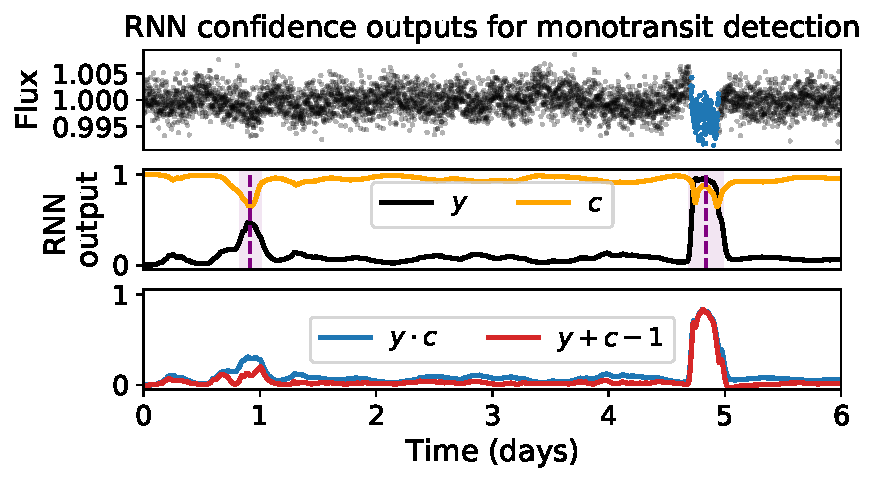
\includegraphics[width=0.5\linewidth]{Experiments/Figures/Monos/mono_example.pdf}
    \caption{An example of how the RNN outputs could be used for monotransit detection. The standard outputs $y$ define the PTS for the given input, which can directly be used to set a threshold on candidate detections (e.g. purple shows candidate detections for $y >0.25$). In case the confidence RNN is used we also get $c$, which we use in two ways in combination with $y$ to define an alternative PTS with the aim of reducing peaks for which the RNN is less certain. These curves, as shown in the bottom panel, can similarly be used to set detection thresholds.}
    \label{fig:mono_example}
\end{figure}

As baseline we use the monotransit detection algorithm used by \cite{foreman2016population}, which is based on a box function that is fitted to the data at different points in time. The only adjustment we made was that instead of searching for transits of a single duration, we combine the detection results from different trial durations ranging from 1 to 13 hours in steps of 1 hour. The output of the algorithm is a time series of SNR values of the best-fitting box at each time step, which we will refer to as SNR-TS. We set a detection threshold on the SNR above the noise floor in the SNR-TS, which is computed using a sliding median filter. Before applying this method, we detrend the input light curves with a sliding median filter with varying window sizes, i.e. 6, 12, and 24 hours. Since the algorithm is similar to BLS, we refer to it as Mono-BLS-\{6h, 12h, 24h\}, where the extension (e.g. ``6h'') refers to the window length of the detrending filter.

Figure \ref{fig:mono_pr} shows the PR-curves of the different detection algorithms. In this experiment, the RNN outperformed Mono-BLS, which can also be seen in Figure \ref{fig:mono_transits} where we take a closer look at the performance of both methods for specific transit samples. Furthermore, the Conf-RNN performed similar to Mono-BLS and thus worse than the standard RNN, even the Conf-RNN that did not make use of its confidence outputs. In other words, the supposedly more intuitive network came at the cost of worse performance. Table \ref{tab:mono_AnotB} presents the exact number of planets retrieved by the best performing methods at a precision of 0.5, including the number of planets found by one method that were not found by the other.

In terms of computational efficiency, the RNN greatly outperformed (our implementation of) Mono-BLS. For the search for monotransits in 5000 light curves, Mono-BLS took about 10 hours on a CPU, while the RNN only took a few minutes on a GPU. If no GPU is available, the RNN would have taken about 2 hours for this task. For Mono-BLS, the computation time could probably be reduced to a few hours by using less trial durations, using a lower time resolution for the search, or using a faster programming language for the implementation. However, since the RNN can generally easily be run on a GPU, if available, with a library such as PyTorch, and pre-implemented algorithms such as (Mono-)BLS do not naturally come with GPU compatibility, the RNN remains the preferred choice in terms of efficiency.

\begin{figure}
    \centering
    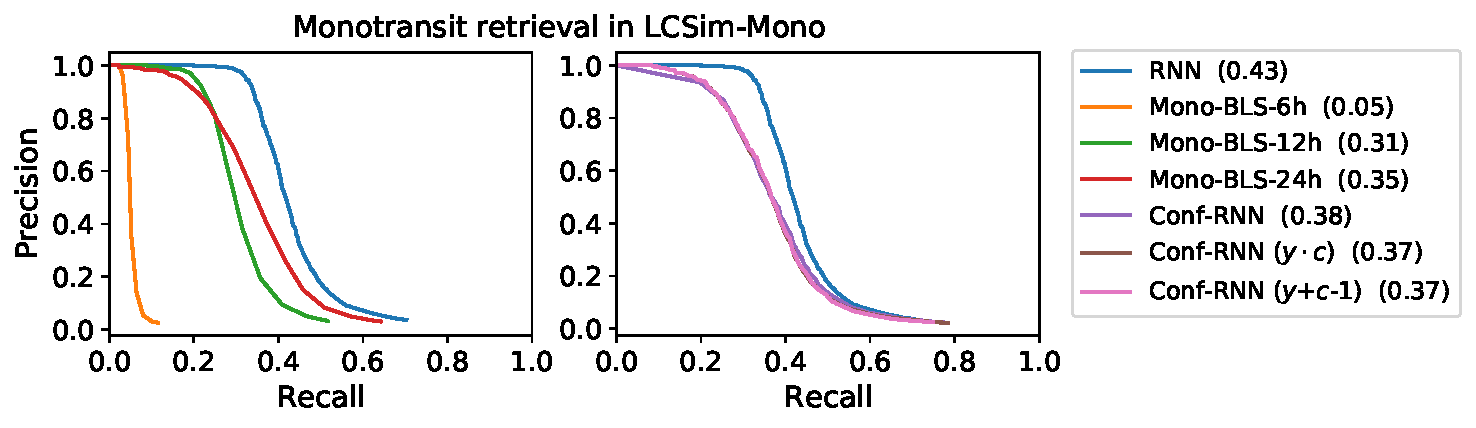
\includegraphics[width=0.8\linewidth]{Experiments/Figures/Monos/mono_pr.pdf}
    \caption{Precision-recall (PR) curves of different methods in the task of monotransit detection, divided over two figures to avoid clutter. The area under the curve, or average precision (AP), is given between brackets for each method. The RNN is the single-layer bi-GRU which only outputs the PTS for a given input light curve. Conf-RNN is a network which outputs confidence values in addition to the standard PTS, which performed worse than the standard RNN, even if the confidence values are not used.}
    \label{fig:mono_pr}
\end{figure}

\begin{figure}
    \centering
    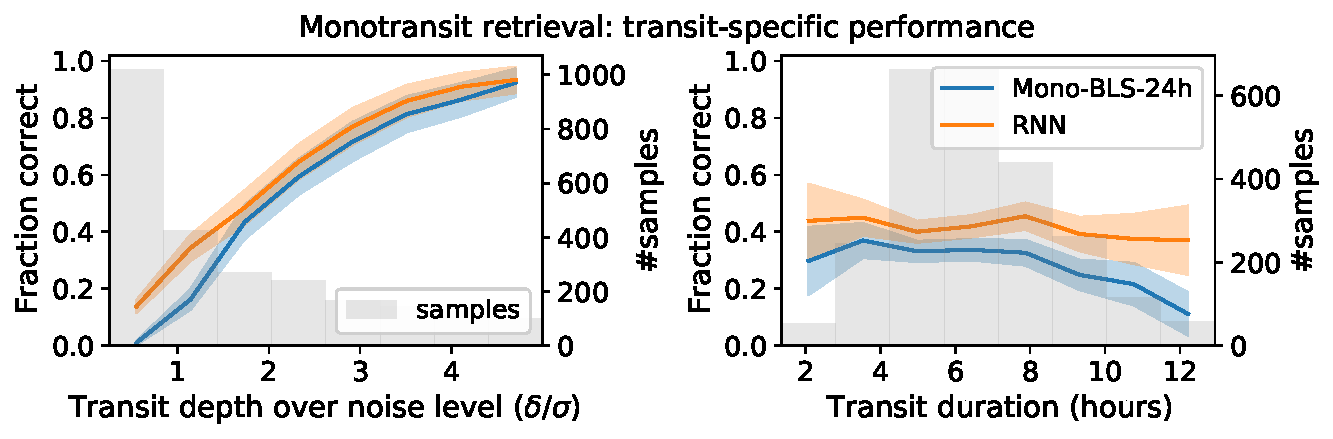
\includegraphics[width=0.7\linewidth]{Experiments/Figures/Monos/mono_transit_specific.pdf}
    \caption{A close in on the ability of the presented methods to retrieve specific transit samples, e.g. if the fraction correct is 0.5, then half of the planets were detected in the corresponding parameter bin. Underlying data distributions are shown in gray which also indicate the bins used in the evaluation. The detection threshold for both methods was set closest to a corresponding detection precision of 0.5. Filled regions show the Wilson score interval \citep{wilson1927probable} which approximates the 95\% confidence interval of the performance within each bin.}
    \label{fig:mono_transits}
\end{figure}

\begin{table}[]
\label{tab:mono_AnotB}
\centering
\begin{tabular}{@{}lrlrl@{}}
\toprule
                 & \multicolumn{2}{c}{RNN} & \multicolumn{2}{c}{Mono-BLS-24h} \\ \midrule
                 & 1042   & (1.00, 0.42)   & 818        & (1.00, 0.33)        \\
not RNN          & -      &                & 74         & (0.09, 0.03)        \\
not Mono-BLS-24h & 298    & (0.29, 0.12)   & -          &                     \\ \bottomrule
\end{tabular}
\caption{The absolute and relative number of correct detections in the task of retrieving monotransits, where the detection thresholds are set closest to a corresponding detection precision of 0.5. An element, say with labels ``A'' in the corresponding column and ``not B'' in the row, corresponds to the number of detected planets by A that are not detected by B. Values between brackets respectively show the fraction with respect to the total number of detections of A, and the fraction with respect to the total amount of planets in the data, i.e. 2500.}
\end{table}
